% PART IV — PHASE-WISE RESEARCH AND IMPLEMENTATION
\chapter{Chapter 5: Early Foundations Through Sparse Deadlocks (Phases 1–11)}
\section{5.1 Reconstructed History of Phases 1–8 (Git \& Telemetry Evidence)}
Phases 0 and 1 (commits 3a345f3, a5cc06b, 7ad9848 on 2026-10-03) built URDF modeling, PyBullet 240 Hz stepping, and damped least-squares IK, verifying 0.7–4.5 mm accuracy across 5 waypoints (37/37 tests in 4.71 s). Phases 2–4 implemented `PandaReachEnv`, SB3 SAC+HER callbacks, and `PandaPickEnv`. Note on historical provenance: standalone Phase 5 markdown logs and isolated pre-squash Phase 2 vs Phase 3 commits are NOT RECOVERABLE FROM AVAILABLE EVIDENCE and are never extrapolated beyond verified TensorBoard runs (`reach\_sac/SAC\_3`, `pick\_sac/SAC\_1`) and scripted benchmarks (Reach Step 6, Pick Step 67).

Phase 6 (`PandaPickPlaceEnv`) resolved `ERR-001` (finger pad `lateralFriction=2.0`, `spinningFriction=0.1`) and contrasted E1 (No-HER: 7.7 table collisions/ep, actor loss +17.767) against E2 (`HER k=4`: 0.0 collisions, actor loss +2.594) across 10k smoke runs (Figure 5.1). Phases 7–8 scaled to colored `SortingBin` tasks (`Sort` Step 79, `MultiSort` Step 209, `Assembly` Step 143 scripted). Phases 9–10 repaired lazy simulation connection `client\_id=-1` in `PandaAssemblyEnv.reset()` (`ERR-002`, 52/52 tests) and verified scripted DR R0–R4 (75–100\%).

\begin{figure}[htbp]\centering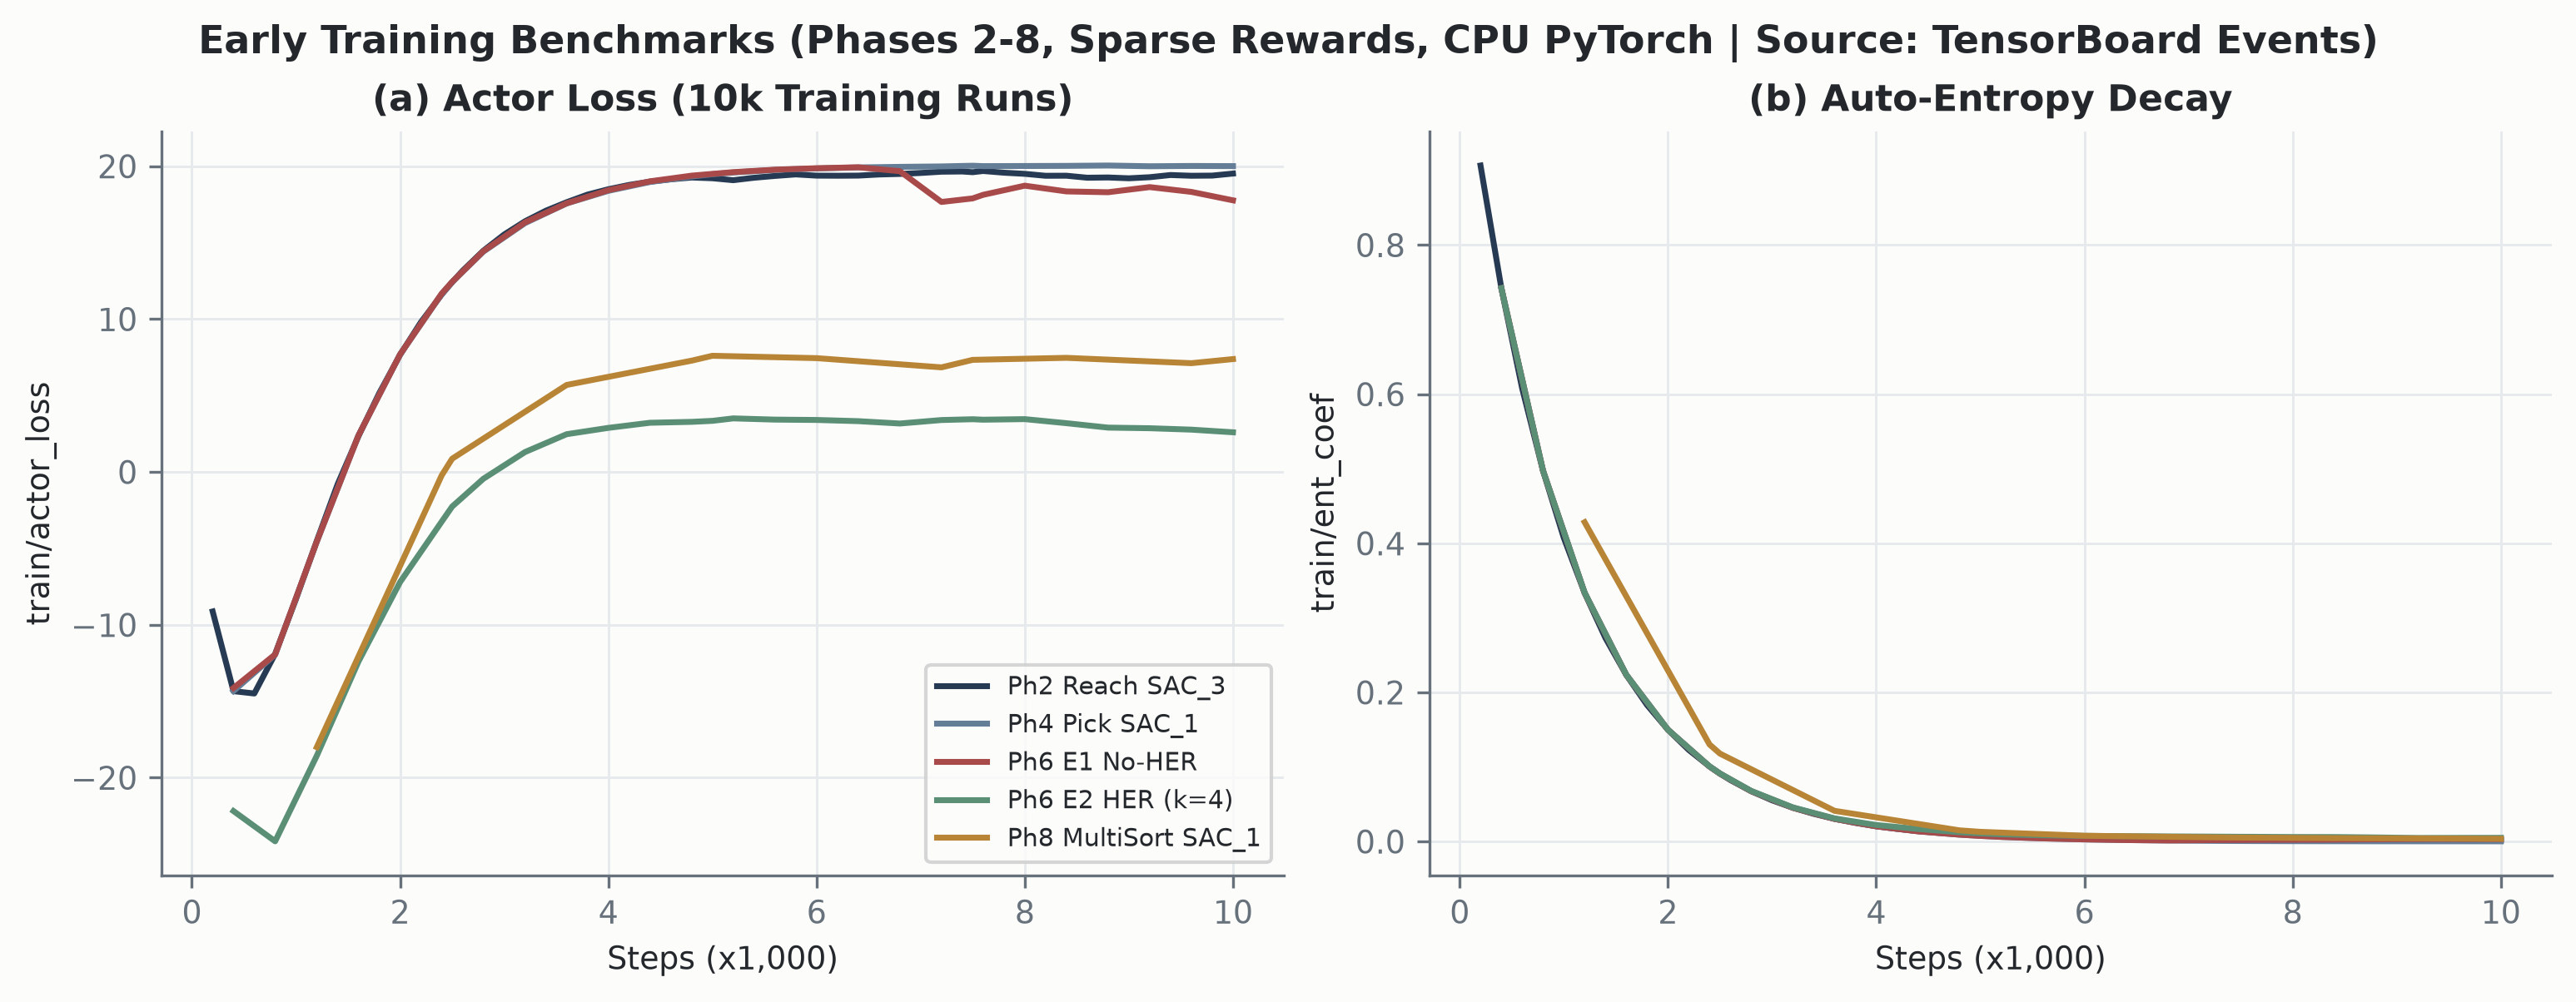
\includegraphics[width=0.9\linewidth]{../../assets/plots/plot_01_early_tb_curves.png}\caption{Figure 5.1: Reconstructed Phases 2–8 TensorBoard actor loss and entropy coefficient decay trajectories (CPU PyTorch, 10k runs).}\end{figure}
\section{5.2 Phase 11: Systematic Diagnosis of the Sparse HER Equilibrium (2.5M Steps)}
Evaluating 25 sparse SAC+HER models (5 DR tiers x 5 seeds, 100k steps each; 5,000 total evaluation episodes) produced uniformly 0.0\% completion across both Nominal and Held-Out DR4 splits (Figure 5.2). Isolating transport via `TransportDiagnosticEnv` (Phase 11.9) proved 100.0\% transport convergence in 40k–50k steps (0.009 m error), demonstrating that sparse reward failure stemmed strictly from initial grasp acquisition starvation rather than spatial goal transport capacity.

\begin{figure}[htbp]\centering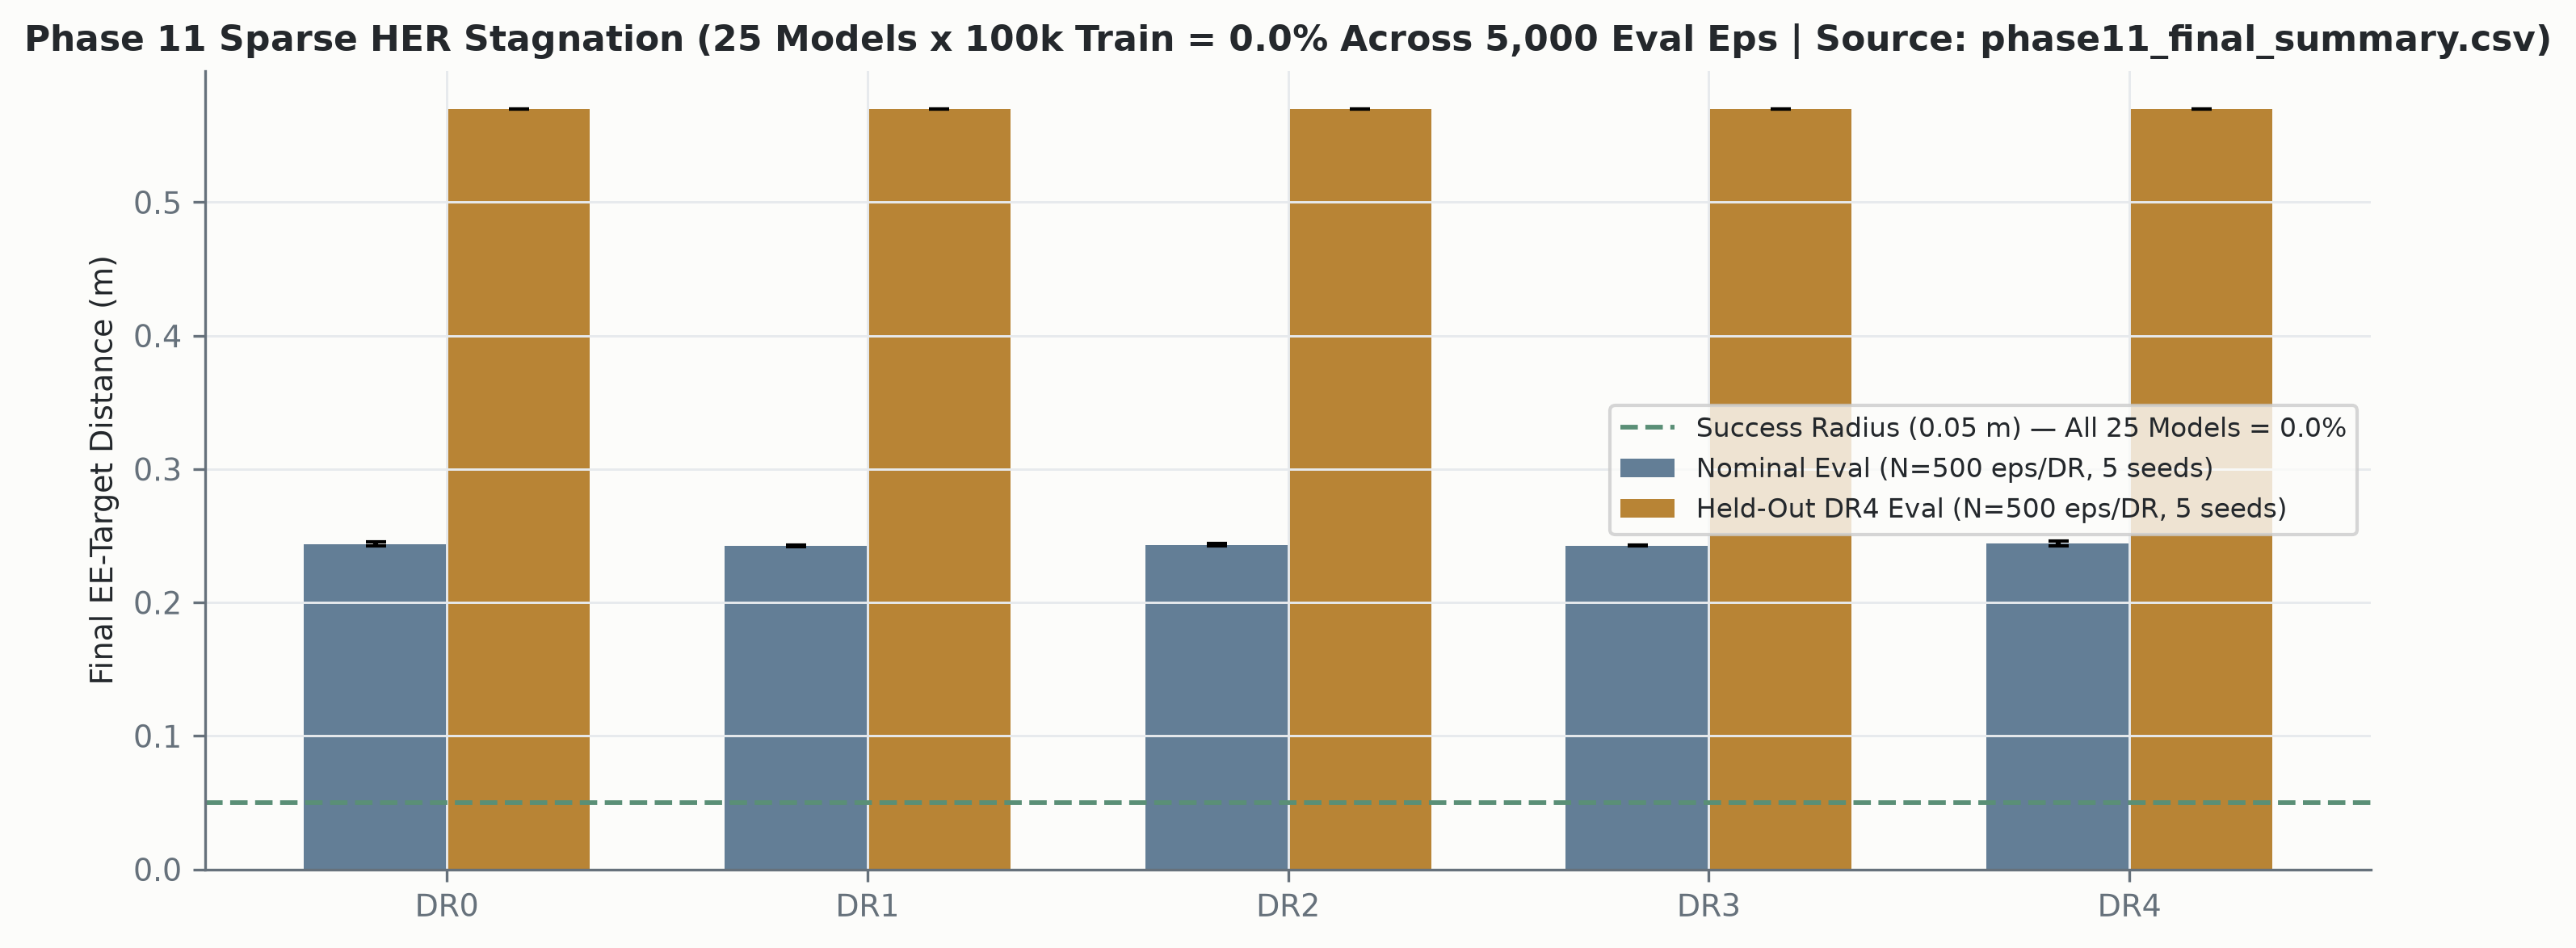
\includegraphics[width=0.9\linewidth]{../../assets/plots/plot_02_phase11_sparse_vs_transport.png}\caption{Figure 5.2: Phase 11 25-model sparse stagnation across 5,000 evaluation episodes (Mean +/- SD across 5 seeds per DR tier).}\end{figure}